
\documentclass[aspectratio=169]{beamer}
\usetheme{metropolis}           % Use metropolis theme
\usepackage[utf8]{inputenc}
\usepackage{graphicx}
\usepackage{eso-pic}
\usepackage{graphics}
\usepackage{tikz}
\usepackage[export]{adjustbox}
\usepackage{multicol}
\usepackage{listings}
\usepackage{helvet}
\usepackage{booktabs}
\usepackage{threeparttable}


\title{Reproducible Randomization}
\date{\today}
\author{Benjamin Daniels} % Name of author(s) of session here
\institute{Development Impact Evaluation (DIME) \newline The World Bank }
\setbeamercolor{background canvas}{bg=white}	% Sets background color

% The below command places the World Bank logo and DIME logo to the right corner
\titlegraphic{%
	\begin{picture}(0,0)
	\put(330,-180){\makebox(0,0)[rt]{
\includegraphics[width=3cm]{img/WB_logo}}}
	\end{picture}%
	\begin{picture}(0,0)
	\put(390,-180){\makebox(0,0)[rt]{
\includegraphics[width=1.5cm]{img/i2i}}}
	\end{picture}%
}

%%% Section page with picture of Light bulb
\makeatletter
\defbeamertemplate*{section page}{mytheme}[1][]{
	\centering
	\begin{minipage}{22em}
		\raggedright
		\usebeamercolor[fg]{section title}
		\usebeamerfont{section title}
		\par
		\ifx\insertsubsectionhead\@empty\else%
		\usebeamercolor[fg]{subsection title}%
		\usebeamerfont{subsection title}%
		\fi
		\ifstrempty{#1}{}{%
			\includegraphics[width=100mm, height=60mm]{#1}%
		}
		\insertsectionhead\\[-1ex]
		\insertsubsectionhead
		\usebeamertemplate*{progress bar in section page}
		
	\end{minipage}
	\par
	\vspace{\baselineskip}
}
\makeatother

%%% Define a command to include picture in section, 
%%% make section, and revert to old template
\newcommand{\sectionpic}[2]{
	\setbeamertemplate{section page}[mytheme][#2]
	\section{#1}
	\setbeamertemplate{section page}[mytheme]
}

%%% The command below allows for the text that contains Stata code
\lstset{ %
	backgroundcolor=\color{white},
	basicstyle=\tiny,
	breakatwhitespace=false,
	breaklines=true,
	captionpos=b,
	commentstyle=\color{green},
	escapeinside={\%*}{*)},
	extendedchars=true,
	frame=single,
	numbers=left,
	numbersep=5pt,
	numberstyle=\tiny\color{gray},
	rulecolor=\color{black},
	showspaces=false,
	showstringspaces=false,
	showtabs=false,
	stringstyle=\color{mauve},
	tabsize=2,
	title=\lstname,
	morekeywords={not,\},\{,preconditions,effects },
	deletekeywords={time}
}

%% The below command creates the ligh bulb logos in the top right corner of the 
\begin{document}
	
{
	\usebackgroundtemplate{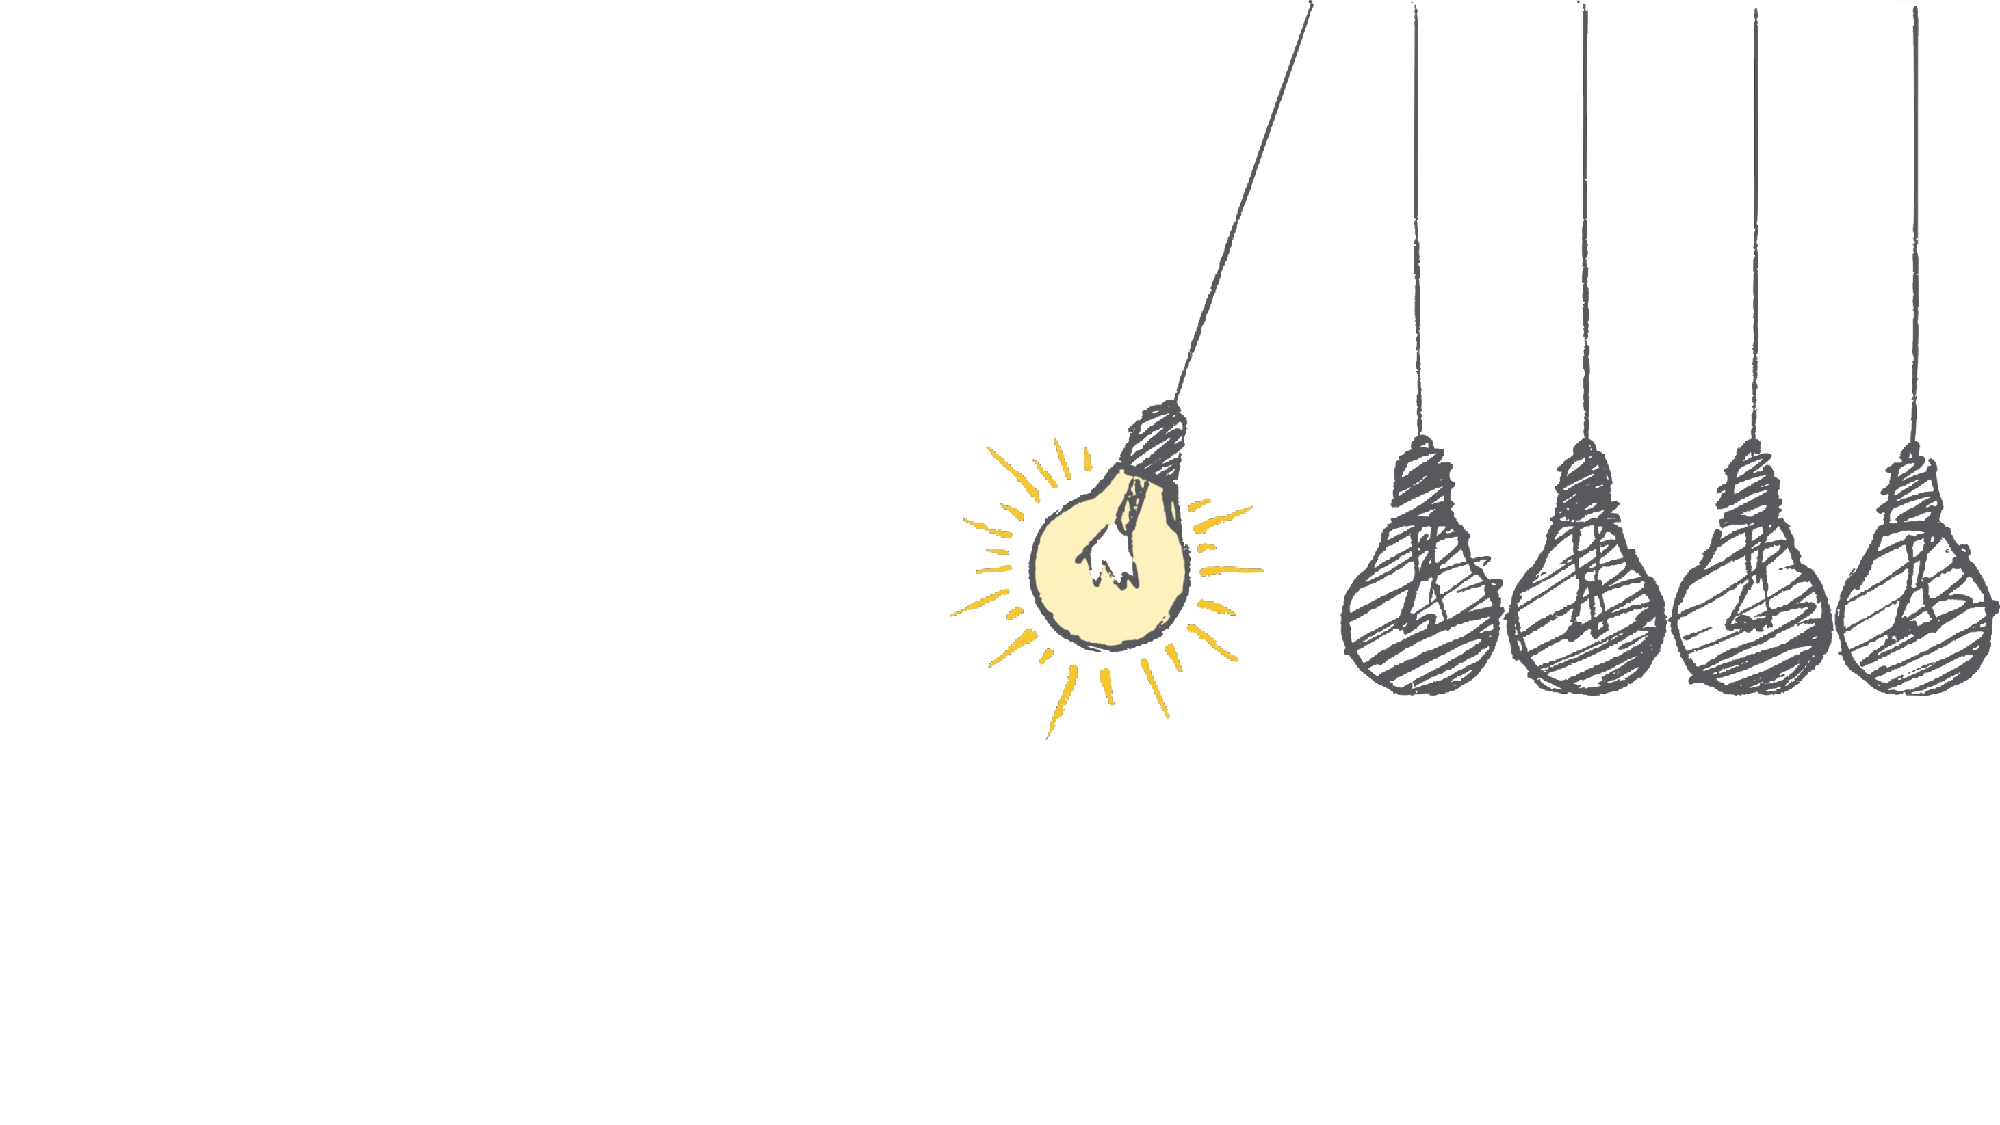
\includegraphics[height=55mm, right]{img/top_right_corner.pdf}}
	\maketitle
}

\begin{frame}{Why do we randomize?}

	\begin{itemize}[<default overlay specification>]
		\item<1> We want to assign the intervention of our projects so that the control group is as similar as possible to the treatment group as possible. 
			\newline - This is called a balanced treatment assignment. 
			\newline - Randomization is the most common tool to achieve that.
			\newline - With randomization, we know that the treatment is uncorrelated with the outcome ex ante.
		\item<1> Each observation needs to have the same probability to end up in the each treatment arm, and all groups need to be statistically similar. 
	\end{itemize}

\end{frame}


\begin{frame}{Background?}

\begin{itemize}[<default overlay specification>]
	\item<1> Pure random assignment guarantees that the treatment and control groups, on average, will have identical characteristics. 
	\item<1> In any particular random allocation, the two groups will differ along some dimensions, with the probability that such differences are large, falling with sample.
		\newline - Confounders. 
		\newline - Efficiency (e.g. unequal group size). 
	\item<1> Small-scale experiments (30 to 100 observations). 
	\item<1> What options exist and what to do?
\end{itemize}

\end{frame}


\begin{frame}[fragile]{Review: Balance tries to establish a counterfactual}
\begin{multicols}{2}	
	
	\textbf{What we know:}
	\newline Good randomization methods produce an unbiased estimate for treatment in the average randomization.
	
	\textbf{What we don’t know:}
	\newline Good randomization methods produce an unbiased estimate for treatment in the average randomization.
	
	\begin{figure}
		\centering
		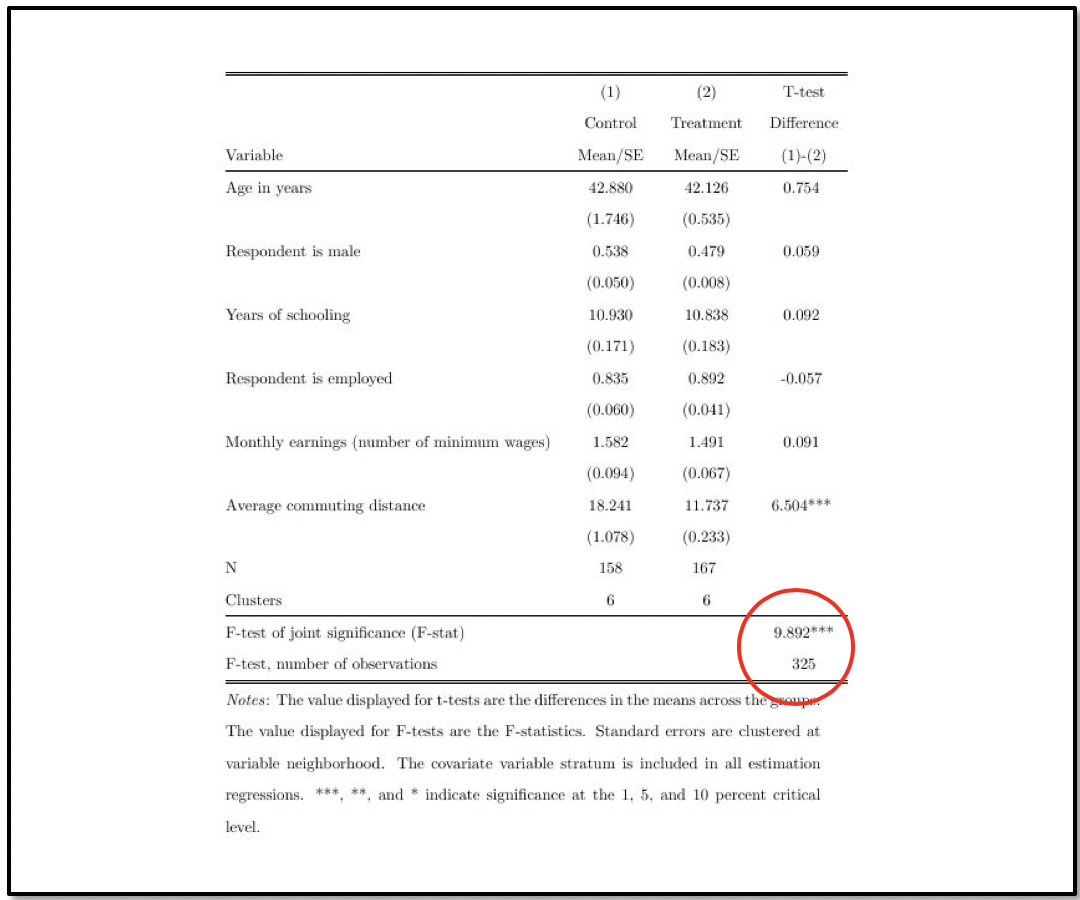
\includegraphics[width=75mm]{img/Balance}
	\end{figure}
	
\end{multicols}
\end{frame}


\begin{frame}{Pure RCTs are balanced – in the average assignment}

\begin{itemize}[<default overlay specification>]
	\item<1> No matter what statistics you are going by, if a (conditional) means difference has p=0.05, a difference of that size will be realized in 5\% of draws. That’s the definition.
	\item<1> The average randomized treatment assignment produces statistically identical groups across treatments.
	\item<1> But, a p=0.05 tail draws happen one time in 20. 
	\item<1> You only get one draw on your randomization!
	\item<1> We’d like balance tests to show ours was a “good” one, so that “real” differences must be due to treatment assignment.
\end{itemize}

\end{frame}


\begin{frame}{Balance leads to unbiasedness: Need a model and an assumption}

\begin{itemize}[<default overlay specification>]
	\item<1> Model – Asymptotically normal OLS
		\newline - T-statistics of “closeness” to the average randomization depend on large-sample properties.
	\item<1> Assumption – no omitted variables in regression
		\newline Unless all x’s in X are in the model, balance on observables doesn’t imply that expected outcomes for treated and untreated are equal.
		\newline If you are wrong, biases are of unknown magnitude and direction depending on the omitted variable’s actual correlation with treatment and outcome variables (classical OVB).
		\newline In small samples especially, can’t guarantee that treatment randomization  produces zero expected differences for all omitted covariates.
\end{itemize}

\end{frame}


\begin{frame}[fragile]{What we often do: block/stratify the experiment}
\begin{multicols}{2}	
	
\begin{itemize}[<default overlay specification>]	
	\item<1>  Meets our core criteria:
		\newline - Randomization process is fixed over real data.
		\newline - Counterfactuals (zero treatment effect) has a distribution that can be simulated exactly.
	
	\item<1>  Allows use of “randomization inference” statistics that do not depend on extrapolation from model.
\end{itemize}
	
	\begin{figure}
		\centering
		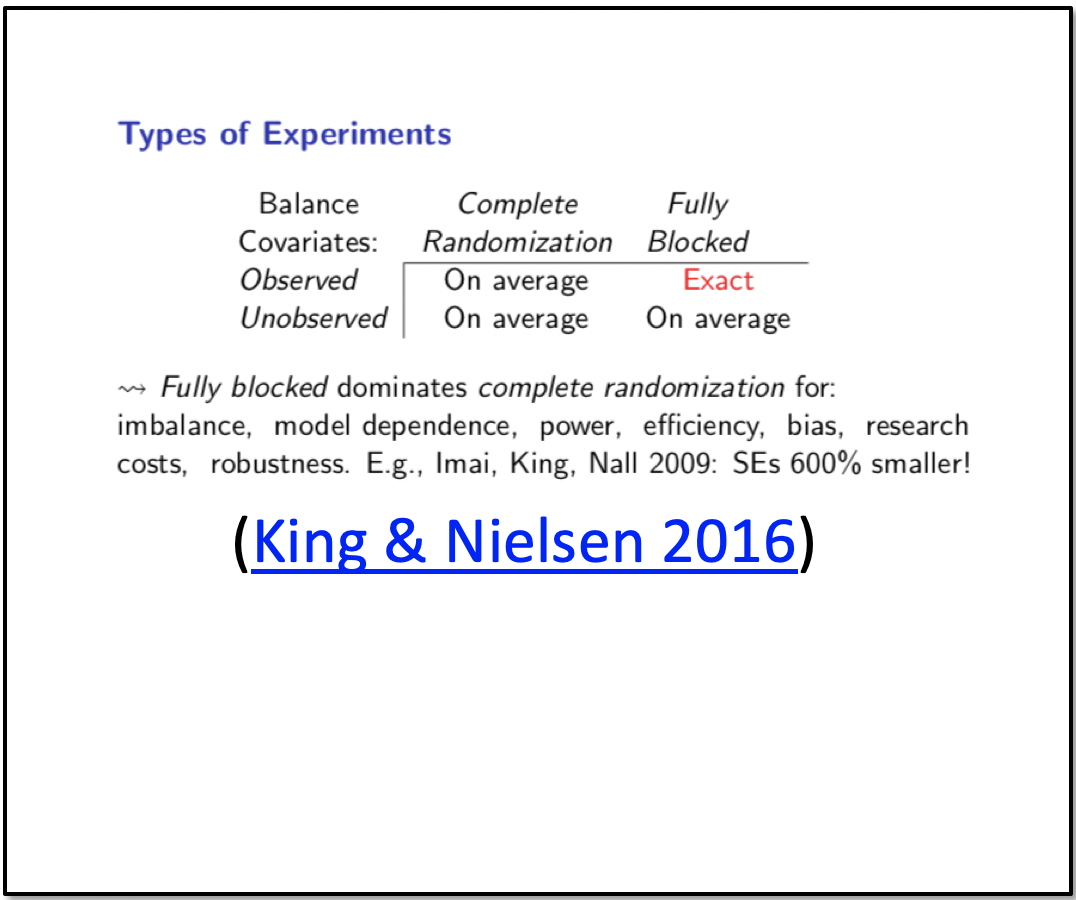
\includegraphics[width=75mm]{img/Balance2}
	\end{figure}
	
\end{multicols}
\end{frame}


\begin{frame}[fragile]{Especially valuable when N is small:}
\begin{multicols}{2}	
	
	\begin{itemize}[<default overlay specification>]	
		\item<1>  Key idea:
		\newline - Reducing the number of possible randomizations to those where the treatment and control are intentionally similar reduces the possible variation in estimate of the true treatment effect.
		\newline - Moderate sample size reduces the advantage, but it depends critically on underlying dispersion of outcomes (Bruhn and McKenzie 2009).
	\end{itemize}
	
	\begin{figure}
		\centering
		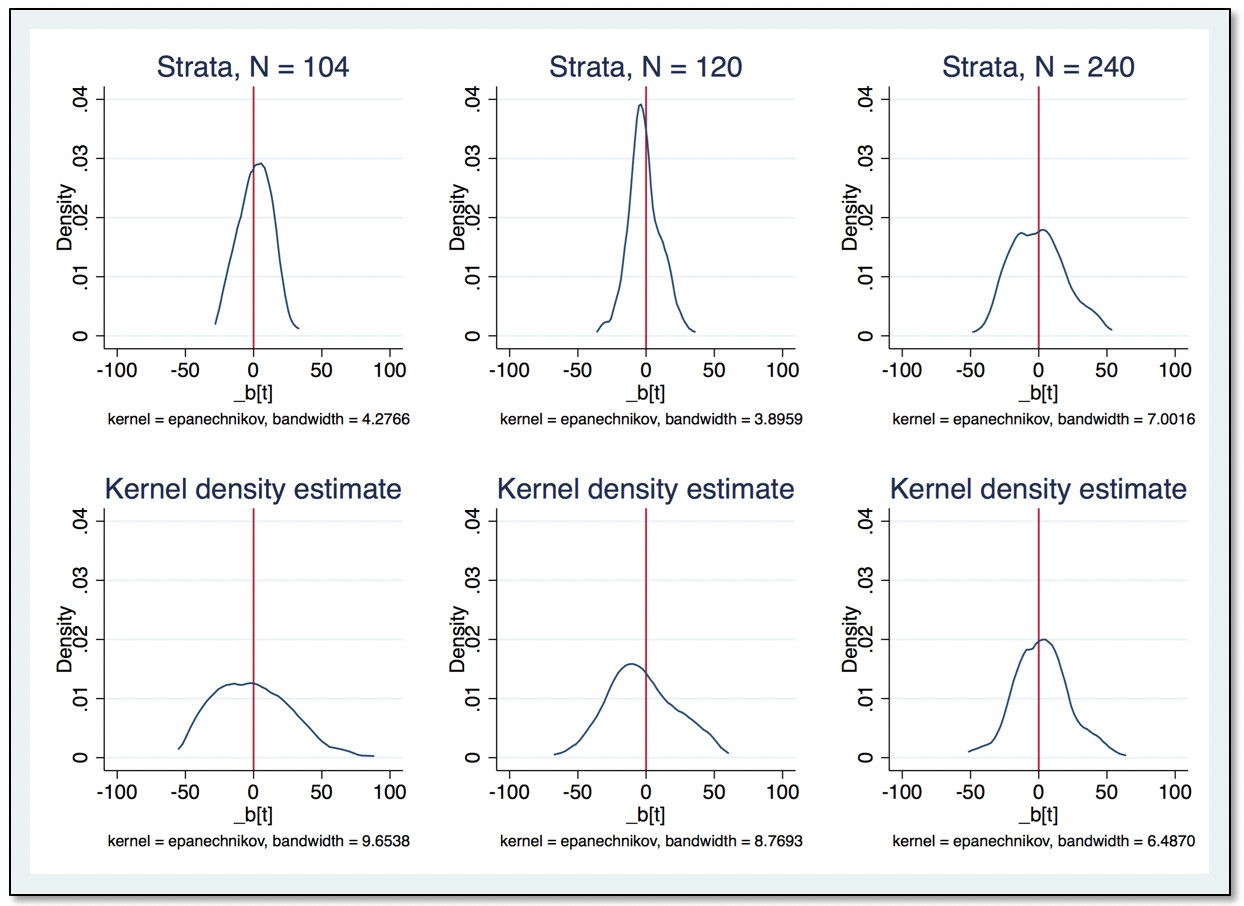
\includegraphics[width=75mm]{img/Small_N}
	\end{figure}
	
\end{multicols}
\end{frame}


\begin{frame}{Types of Randomization}

\begin{itemize}[<default overlay specification>]
	\item<1> Simple
		\newline - Each individual person is assigned either Treatment or Control with some probability.
	\item<1> Cluster
		\newline - Randomization happens on group level (village, school etc. ) and all individuals in a group are assigned the same treatment. 
	\item<1> Stratified
		\newline - Sub-sets of similar observations (rich/poor, male/female etc.) are determined in advance, and randomization is done separately within each sub-set. 
		\newline - Guarantees that equal number of similar observations (rich/poor, male/female etc.) are assigned to be each treatment and control.
	\item<1> Pairwise
		\newline - Extreme form of stratification. 
		\newline - All units are matched to make pairs that are as similar as possible and one unit from each pair is assigned to be T or C.
\end{itemize}

\end{frame}


\begin{frame}{Methods of randomization}

\begin{itemize}[<default overlay specification>]
	\item<1> Good:
		\newline - Field Based.
		\newline -Stata, especially via programming a randomization command. 
		\newline - R, Python, or other replicable software.
	\item<1> Never use:
		\newline - Excel – and other non-replicable software.
		\newline - Excel and many other software has random generators, but they do not allow a controlled randomization. 
\end{itemize}

\end{frame}


\begin{frame}{Randomization: Field vs Computer}
\begin{multicols}{2}	

\begin{figure}
	\centering
	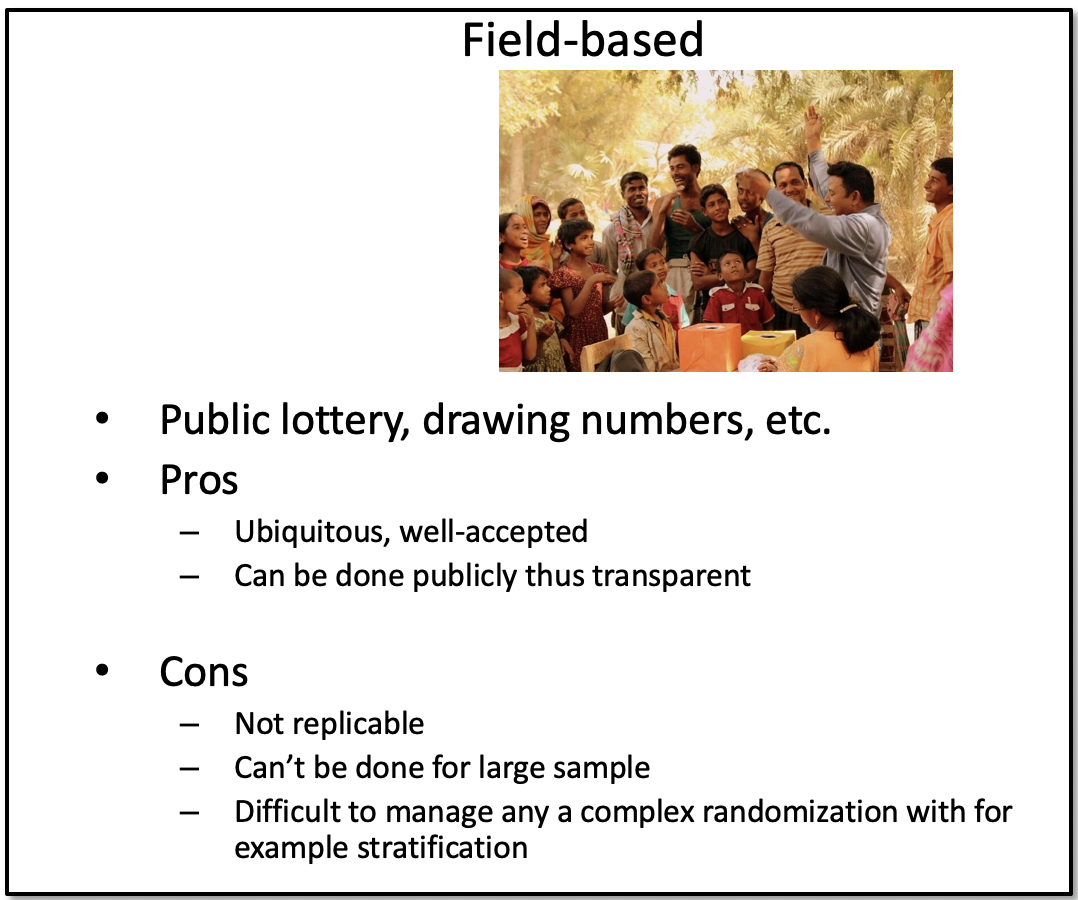
\includegraphics[width=75mm]{img/Randomization}
\end{figure}

\begin{figure}
	\centering
	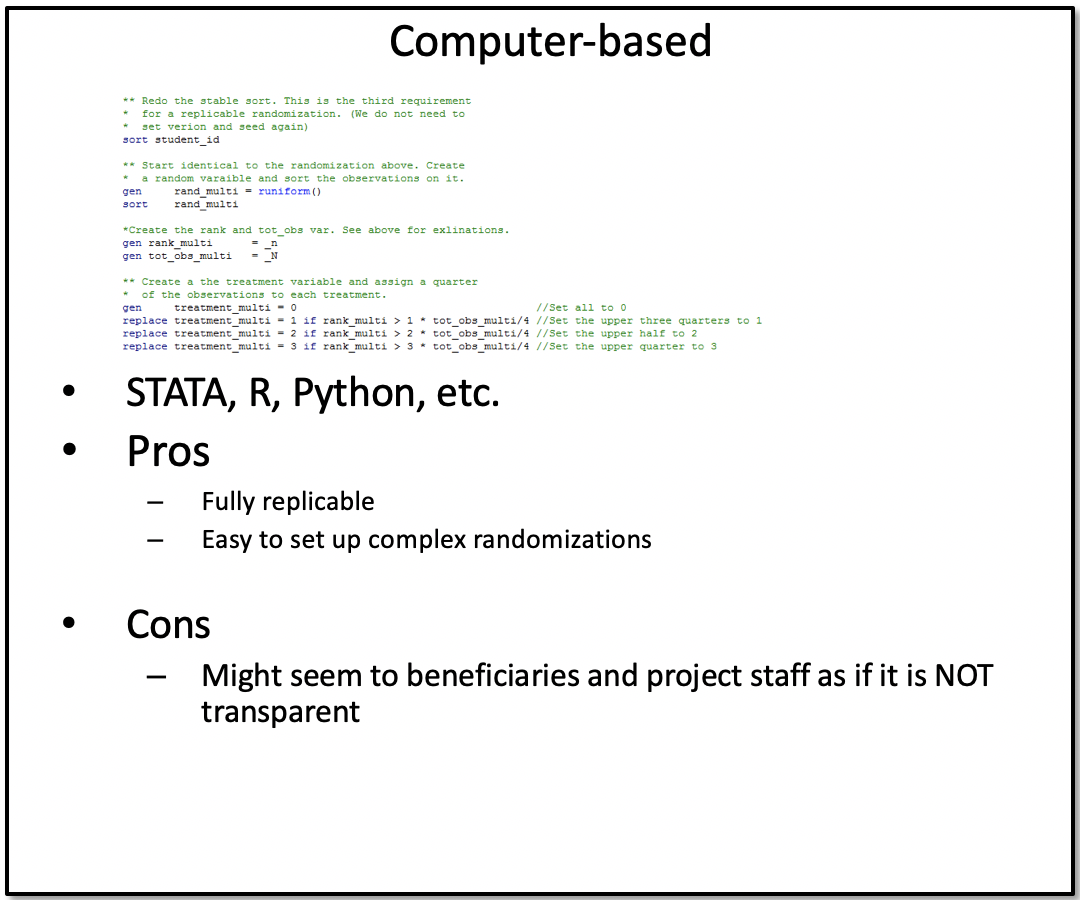
\includegraphics[width=75mm]{img/Randomization2}
\end{figure}

\end{multicols}
\end{frame}


\begin{frame}{Prepare randomization in Stata}

\begin{itemize}[<default overlay specification>]
	\item<1> Define randomization design
		\newline - Unit of randomization (cluster).
		\newline - Number \& size of treatment arms. 
		\newline - Stratification.
		\newline - Variables of interest to test balance.
	\item<1> Obtain a list of observations to be randomized.
	\item<1> Randomize and document using Stata!
\end{itemize}

\end{frame}


\begin{frame}{Ex 1: Basic Randomization in Stata}

\begin{itemize}[<default overlay specification>]
	\item<1> We have 10 students and we want half of them to be treatment and control.
	\item<1> What is our randomization rule?
	\item<1> How do we randomize in Stata such that it is random but replicable?
\end{itemize}

\end{frame}


\begin{frame}[fragile]{Simplified example of randomization}
\begin{multicols}{2}	
	
	\begin{enumerate}[<default overlay specification>]	
		\item<1>  Start with a list of observations you want to randomize. Generate random numbers.
		\item<1> Sort the observations after these random number. The order of the observations are now randomly sorted.
		\item<1> Assign 0 (control) to the first half of the observations, and assign 1 (treatment) to the second half.
	\end{enumerate}
	
	\begin{figure}
		\centering
		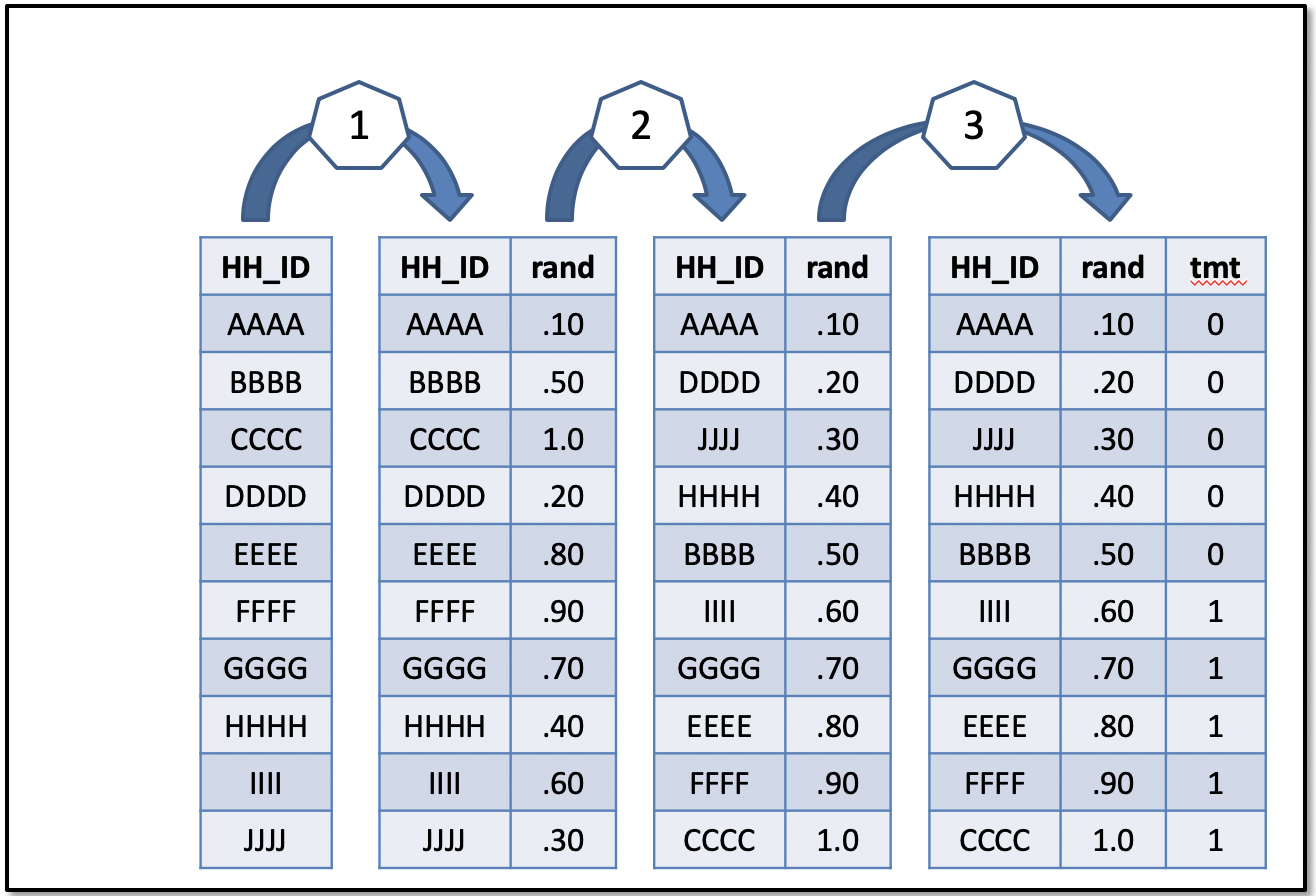
\includegraphics[width=75mm]{img/Randomization3}
	\end{figure}
	
\end{multicols}
\end{frame}


\begin{frame}{The 3 rules of replicable randomization}

\begin{itemize}[<default overlay specification>]
	\item<1> We should make our randomization to be replicable and get the same results for research transparency.
	\item<1> Three rules of replicable randomization in Stata.
		\newline - Same Stata version.
		\newline - Same seed. 
		\newline - Sample ordered in same way.
	\item<1> The next slides explains the meaning of these rules and why it matters.
\end{itemize}

\end{frame}


\begin{frame}[fragile]{Rule 1: Same Stata version}
	
	\begin{figure}
		\centering
		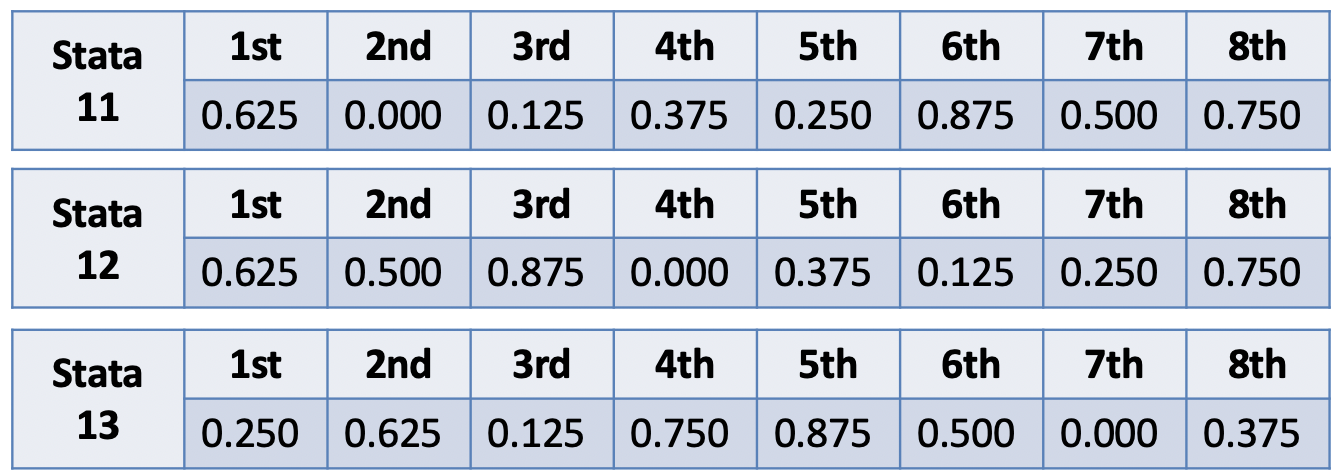
\includegraphics[width=75mm]{img/Randomization4}
	\end{figure}
	
	\begin{itemize}[<default overlay specification>]	
		\item<1>  Stata has pre-calculated list of random numbers. However, each Stata version has a different list of random numbers. 
		\item<1> Any list is equally good for our randomization, but we need to use only one list to get the same result. You can pick one by specifying which Stata version to use in randomization (older version can be used, but not newer). 
		\item<1> In reality these lists are billions of items long, instead of 8 as in the example above. 
	\end{itemize}
	
\end{frame}


\begin{frame}[fragile]{Rule 1: Same Stata version}

\begin{figure}
	\centering
	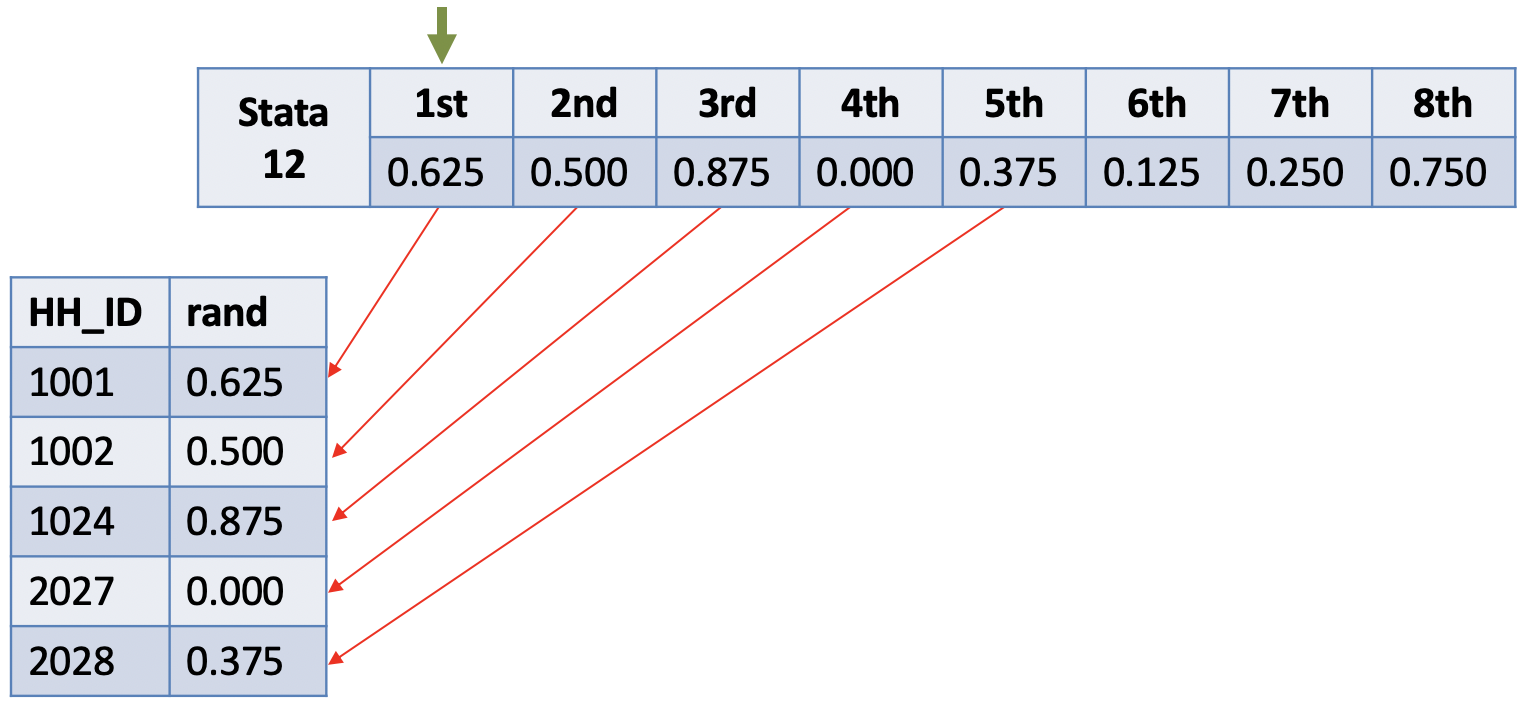
\includegraphics[width=75mm]{img/Randomization5}
\end{figure}

\begin{itemize}[<default overlay specification>]	
	\item<1>  Stata goes through the lists and assigns the 1st value to the first observation, 2nd to the second observation, etc.
\end{itemize}

\end{frame}


\begin{frame}[fragile]{Rule 2: Same seed}

\begin{figure}
	\centering
	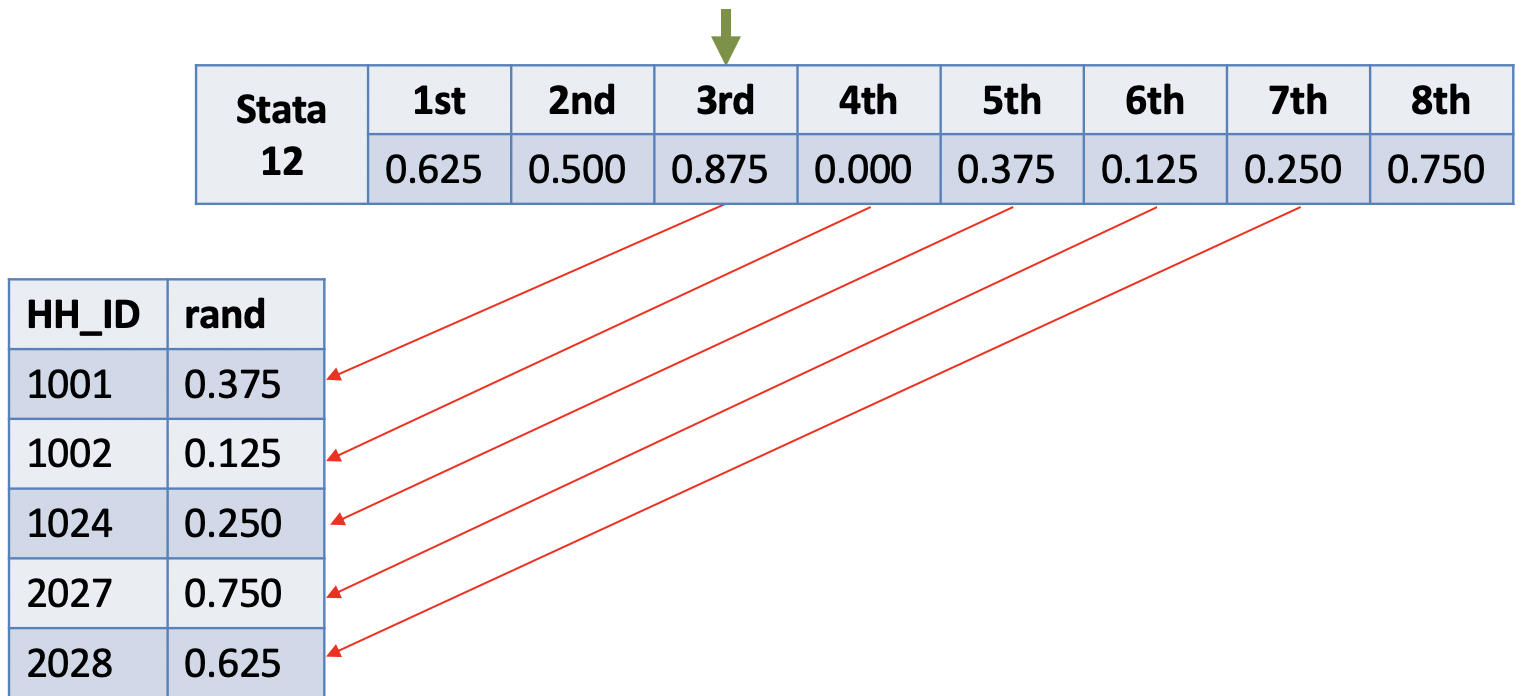
\includegraphics[width=75mm]{img/Randomization6}
\end{figure}

\begin{itemize}[<default overlay specification>]	
	\item<1>  Setting the seed change the starting place in the list.
	\item<1>  Stata has its default seed at the time of launching
	\item<1>  You should set the seed to certain number to make it replicable as well as unique to your study.
\end{itemize}

\end{frame}


\begin{frame}[fragile]{Rule 2: Same seed}

\begin{figure}
	\centering
	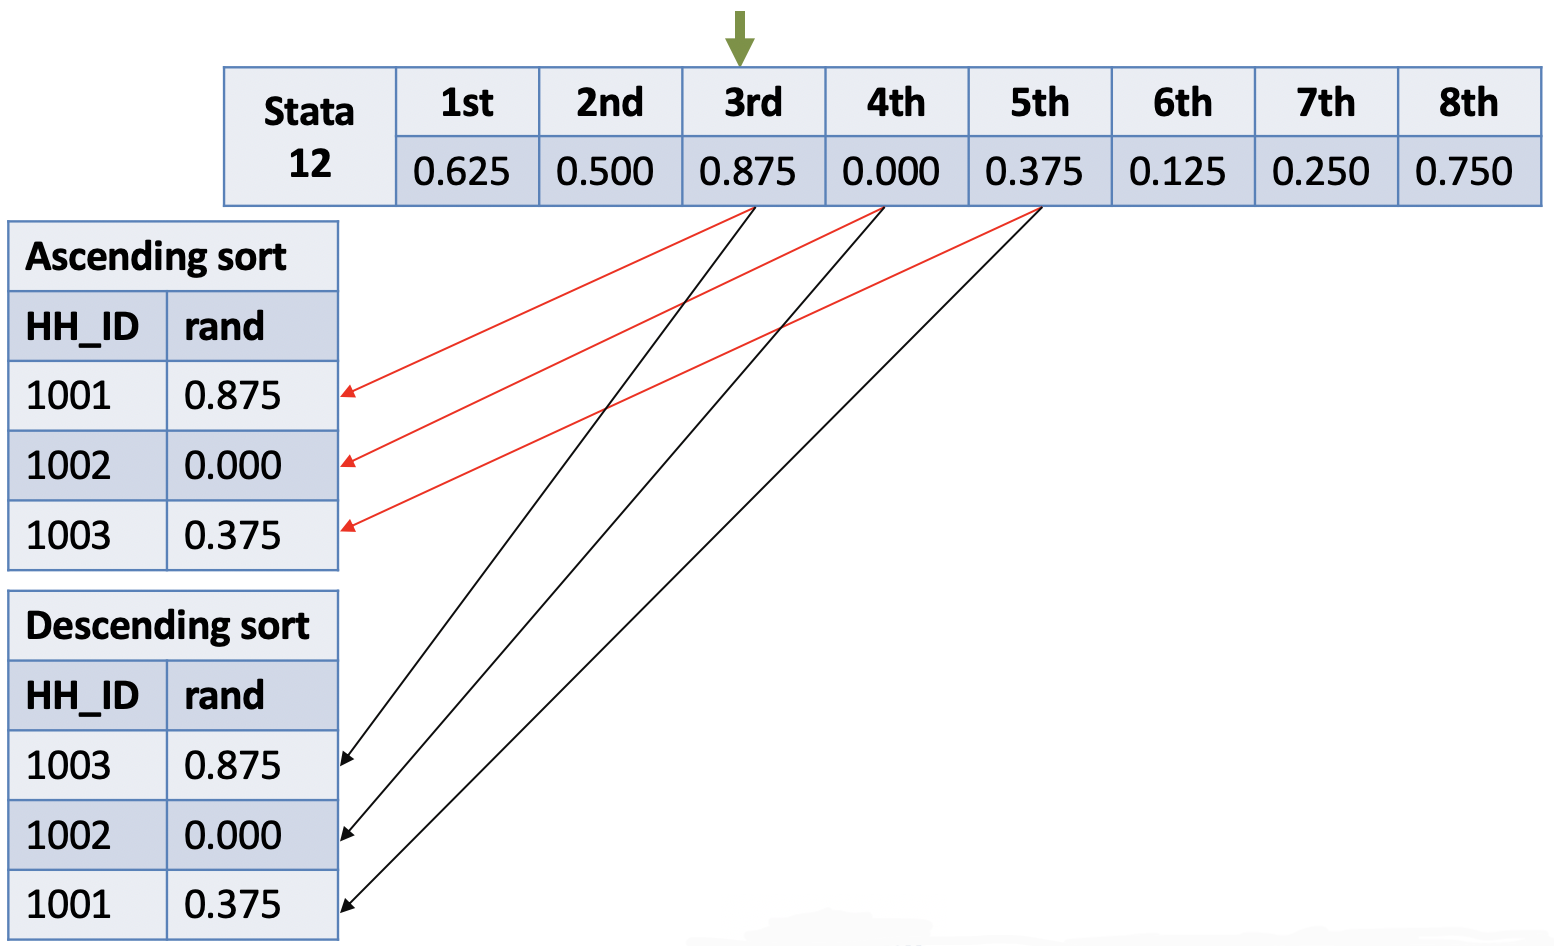
\includegraphics[width=75mm]{img/Randomization7}
\end{figure}

\begin{itemize}[<default overlay specification>]	
	\item<1>  Setting the seed change the starting place in the list.
	\item<1>  Stata has its default seed at the time of launching
	\item<1>  You should set the seed to certain number to make it replicable as well as unique to your study.
\end{itemize}

\end{frame}


\begin{frame}{The 3 rules of replicable randomization]}

\begin{figure}
	\centering
	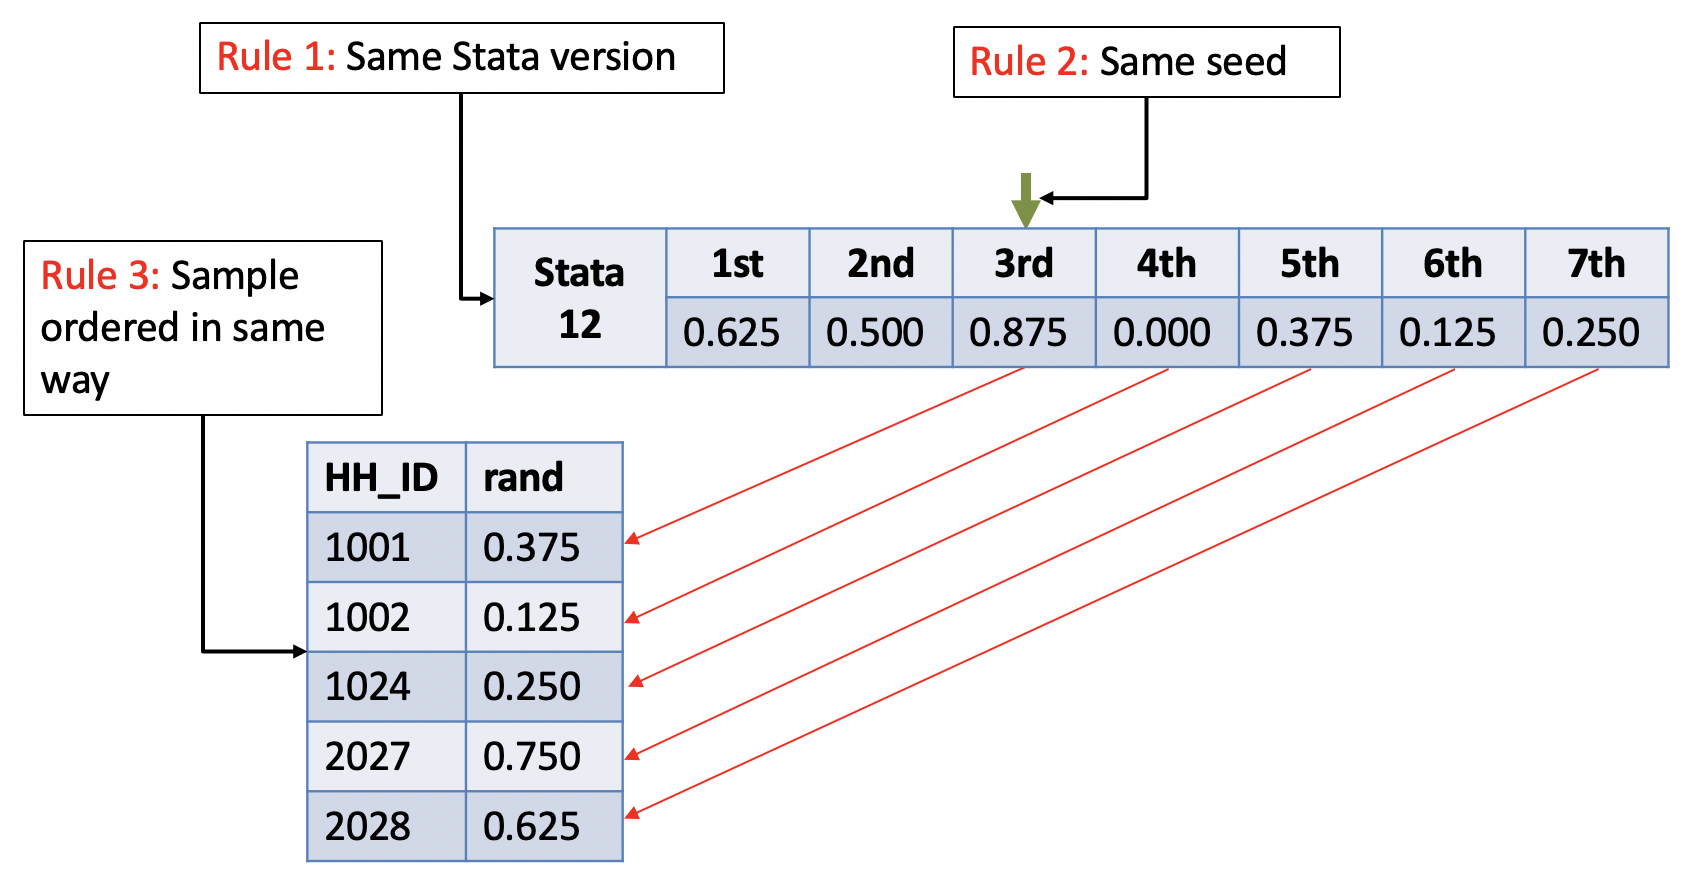
\includegraphics[width=\linewidth]{img/Randomization8}
\end{figure}

\end{frame}


\begin{frame}{The 3 rules of replicable randomization}
\begin{multicols}{2}	

\begin{itemize}[<default overlay specification>]
	\item<1>  Same Stata version.
		\newline - Guarantees the same list.
		\newline - See commands [ieboilstart] or [version] in Stata.
	\item<1>  Same seed.
		\newline - Guarantees the same starting point in the list.
		\newline - Choose a random number outside Stata (ex. random.org).
		\newline - Large number (6-digit or longer) recommended.
		\newline - See command [set seed].
	\item<1>  Sample ordered in same way.
		\newline - Guarantees that the same observation gets the same random number from the list.
		\newline - Sort the data in a way that will remain constant even if someone else change the sort order of the data set you are using (use [isid varlist, sort], NOT [sort varlist, stable]).
		\newline - Be aware that changing the data set, adding or removing observations, changes the sort order and therefore the entire randomization.
\end{itemize}

\end{multicols}
\end{frame}


\begin{frame}{Basic Randomization in Stata}
	
	\begin{itemize}[<default overlay specification>]
		\item<1>  We have 100 students and we want half of them to be treatment and control.
		\item<1>  What are our randomization rules?
		\item<1>  Let’s see an example of a replicable randomization under the given sample and design.
	\end{itemize}
	
\end{frame}


\begin{frame}{Three Rules of Randomization in Stata}

\begin{figure}
	\centering
	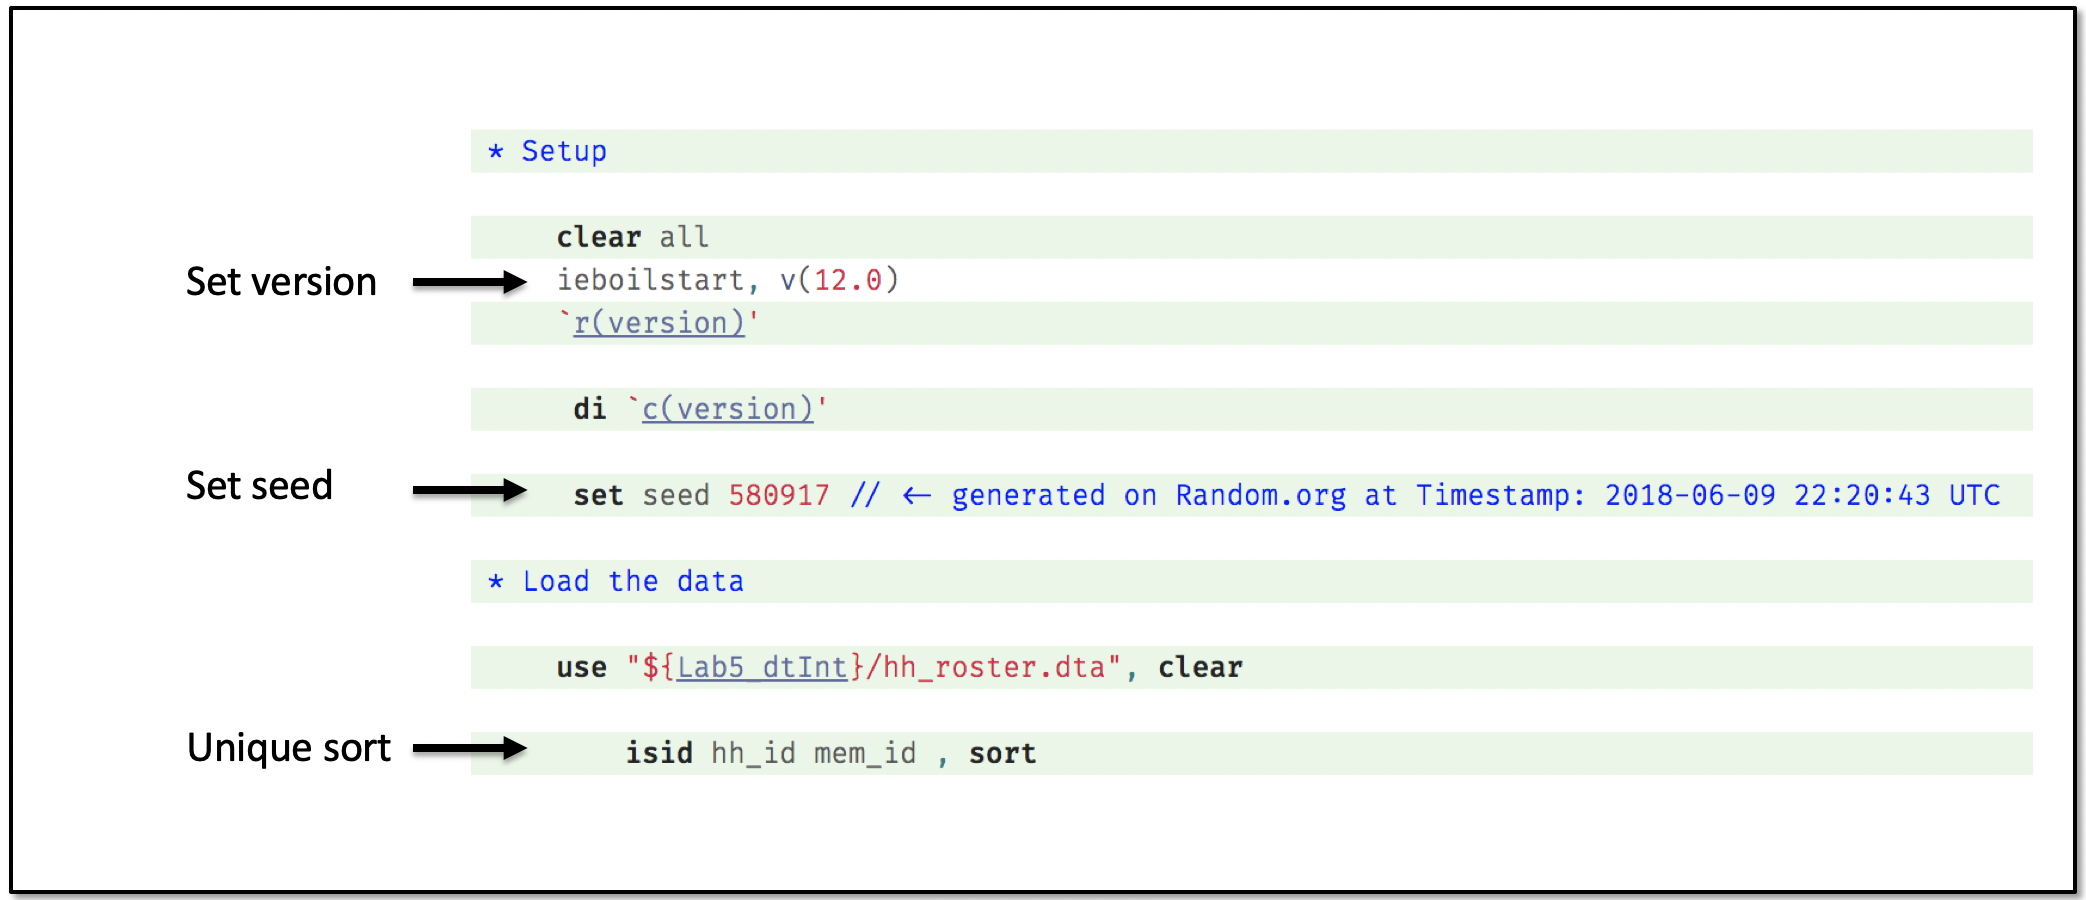
\includegraphics[width=\linewidth]{img/Randomization9}
\end{figure}

\end{frame}


\begin{frame}{Basic Randomization in Stata}

\begin{figure}
	\centering
	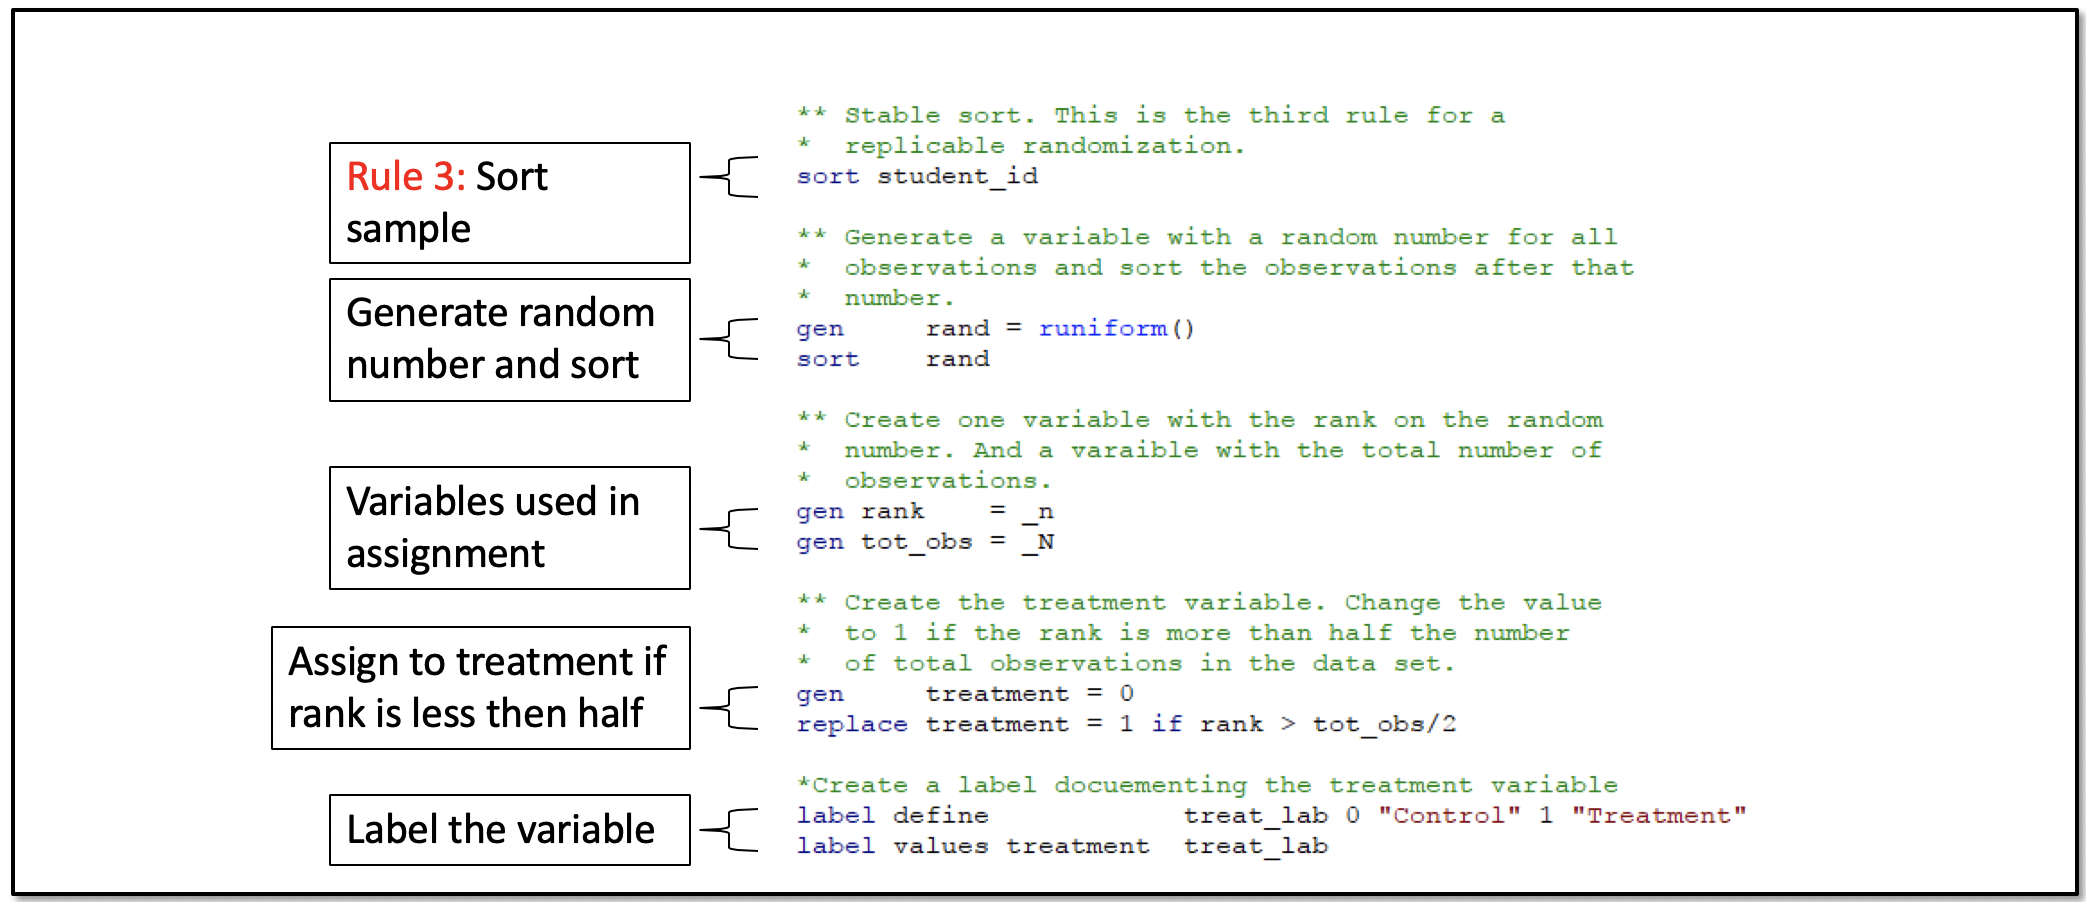
\includegraphics[width=\linewidth]{img/Randomization10}
\end{figure}

\end{frame}


\begin{frame}{Multi-arm randomization in Stata}

\begin{figure}
	\centering
	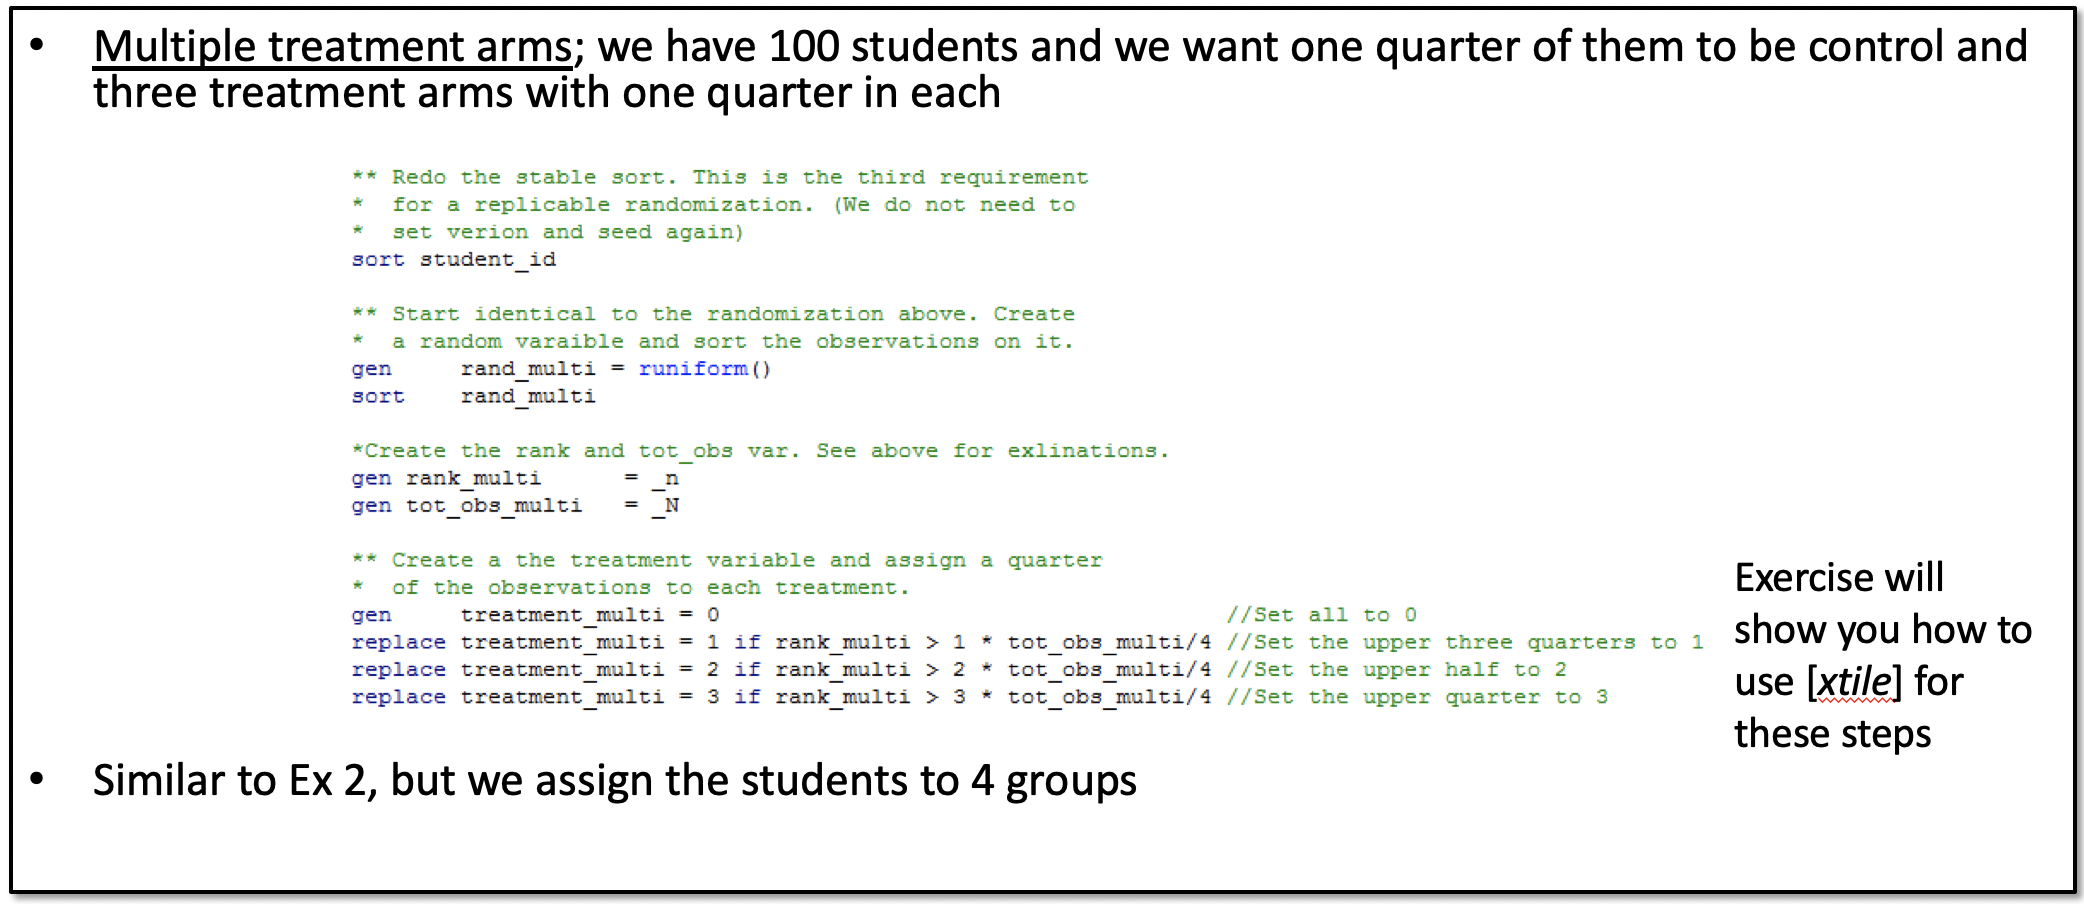
\includegraphics[width=\linewidth]{img/Randomization11}
\end{figure}

\end{frame}


\begin{frame}{Other common randomization}
\begin{multicols}{2}	
	
	\begin{itemize}[<default overlay specification>]
		\item<1>  There are other issues which make randomization more complicated, such as.
			\newline - Groups of different sizes: For example, assigning 40\% to control and 30\% to each of the two treatment arms.
			\newline - Clustering: Randomization is assigned to “clusters” of units at once, such as a household-level treatment.
			\newline - Stratification: Randomization within each subgroup in sample: male/female, rich/poor, regions, etc..
			\newline - Odd total sample size: The number of observations is not evenly divisible with the number of treatment arms in each strata. 
		\item<1>  What kind of code do these require to be random and reproducible?.
		\item<1>  [randtreat] is a user-written Stata command which can help handle all the issues above. We will practice this command in the exercise.
	\end{itemize}
	
\end{multicols}
\end{frame}

%%%%%%%%%%%% heading of section 1 %%%%%%%%%%%%%%%%%%%
\sectionpic{How To Run A Randomization Ceremony}{img/section_slide}

\begin{frame}{Stratified Randomization}

\begin{itemize}[<default overlay specification>]
	\item<1>  Ensures randomization achieves a balance re: several dimensions.
	\item<1>  Example: draw for the World Cup: 32 qualified countries grouped into 4 urns/strata  according to FIFA ranking and assigned to 8 different groups.
\end{itemize}

\end{frame}


\begin{frame}{But first . . . Cluster or stratum?}
\begin{multicols}{2}	
	
	\begin{itemize}[<default overlay specification>]
		\item<1>  Cluster: Units that are grouped and may share similar characteristics; sometimes used as the level of randomization (i.e., treatment assigned v. individual students).
			\newline - The advantage of cluster randomization is that it reduces the likelihood of treatment contamination, but requires more participants to achieve the same statistical power.

		\item<1>  Strata: Groups made up of individuals sharing the same characteristics (i.e., females, males) from which a random sample is drawn.
			\newline - Ensures balance across treatment groups with respect to stratifying variables. Makes it possible to draw inferences about outcomes within each group.
	\end{itemize}
	
\end{multicols}
\end{frame}


\begin{frame}{Examples of clusters}

\begin{figure}
	\centering
	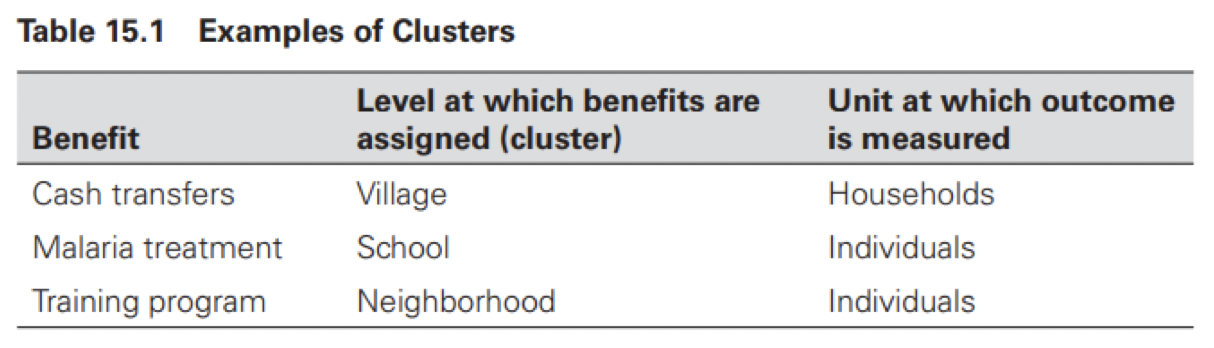
\includegraphics[width=\linewidth]{img/Clusters}
\end{figure}

\end{frame}


\begin{frame}{Stratified Randomization}

\begin{figure}
	\centering
	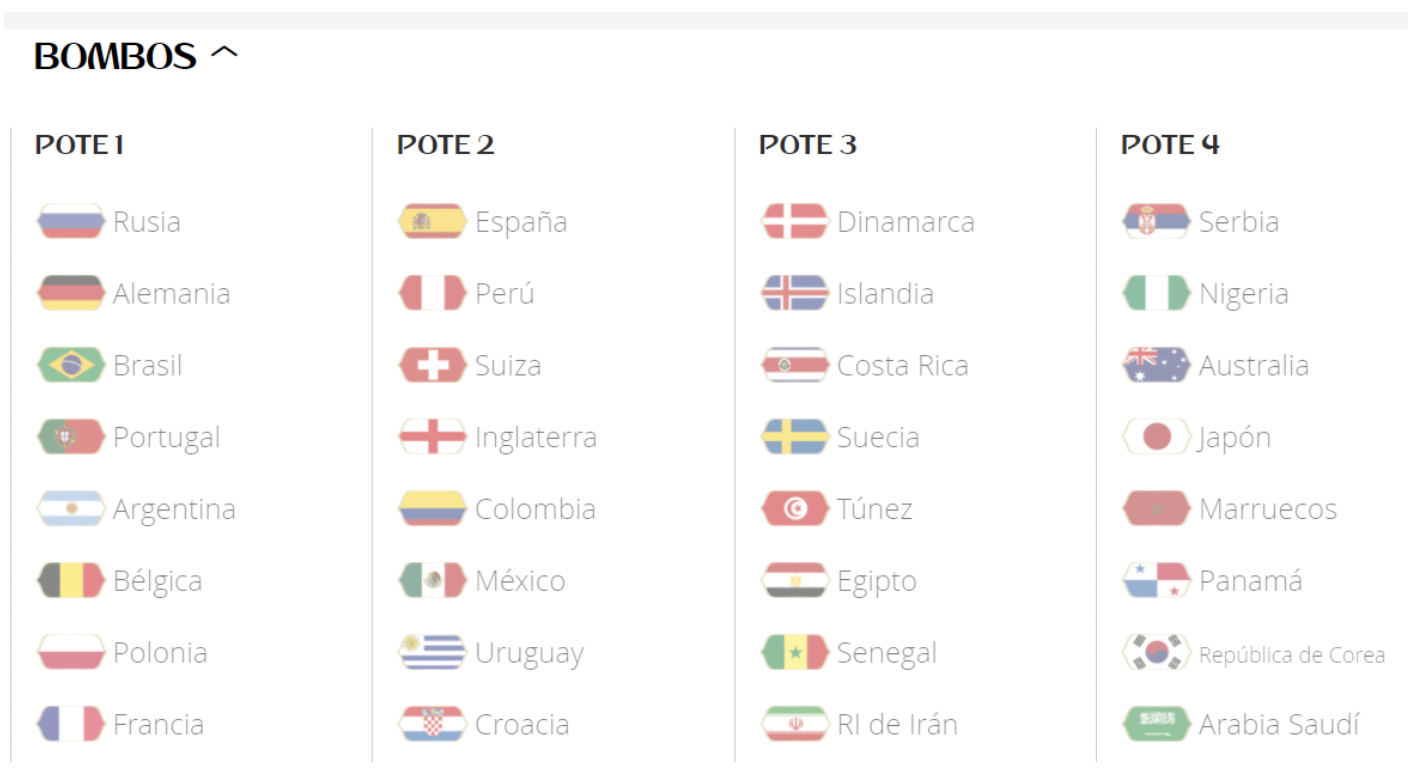
\includegraphics[width=\linewidth]{img/Clusters2}
\end{figure}

\end{frame}


\begin{frame}{Stratified Randomization}

\begin{figure}
	\centering
	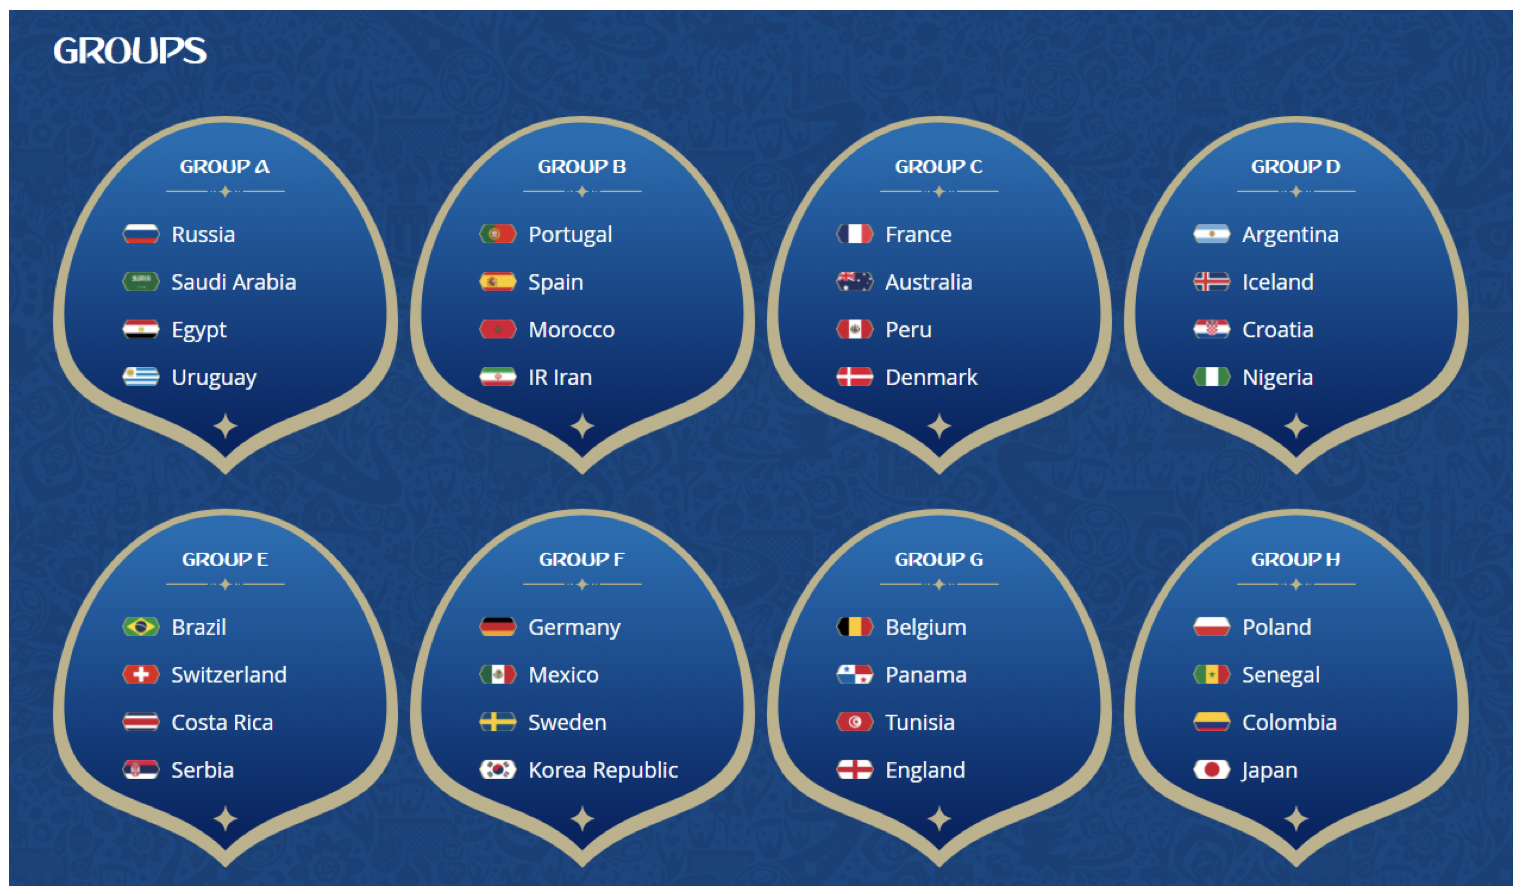
\includegraphics[width=\linewidth]{img/Clusters3}
\end{figure}

\end{frame}


\begin{frame}{Guiding Principles }

\begin{itemize}[<default overlay specification>]
	\item<1>  Maximum number of strata depends on the sample size, the expected size of each strata and the importance of the stratification factors.
	\item<1>  According to simulations, between 22 and 48 strata for a sample size of 100 seems appropriate (individual level randomization). 
	\item<1>  Select covariates that are strongly related to the outcomes of interest, such as geographic region dummies, and variables for which subgroup analysis is desired.
\end{itemize}

\end{frame}


\begin{frame}{Example: Savings, Grants, Training}

\begin{itemize}[<default overlay specification>]
	\item<1>  In the context of new rural roads, we study the impact of complementary interventions for increasing productivity:
	\item<1>  Mechanisms for facilitating access to capital for investment . . .
	
		\begin{figure}
			\centering
			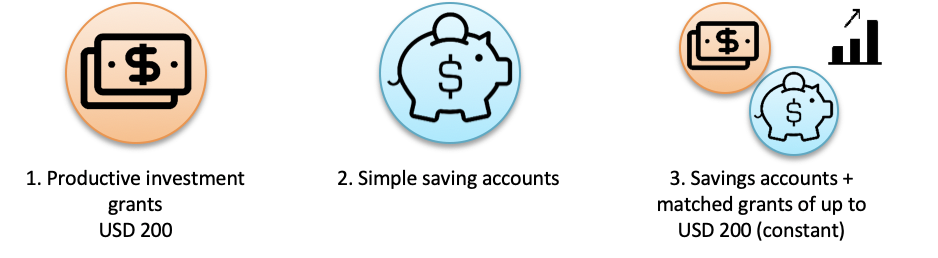
\includegraphics[width=50mm]{img/Grants}
		\end{figure}
	
	\item<1>  Developing the soft skills necessary to be a successful entrepreneur.
	
		\begin{figure}
			\centering
			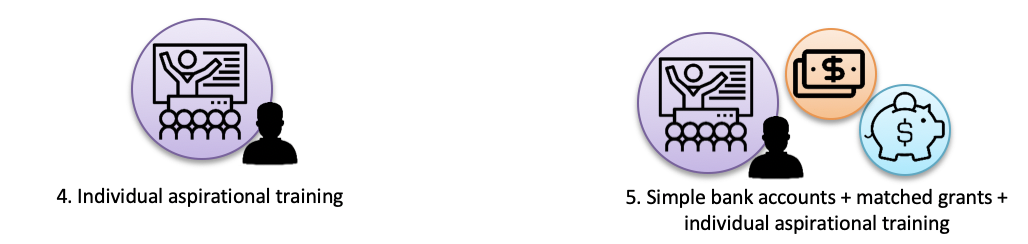
\includegraphics[width=50mm]{img/Grants2}
		\end{figure}
	
\end{itemize}
\end{frame}


\begin{frame}{Example: Savings, Grants, Training}

\begin{itemize}[<default overlay specification>]
	\item<1>  We want to randomize into the following 6 arms.
	
	\begin{figure}
		\centering
		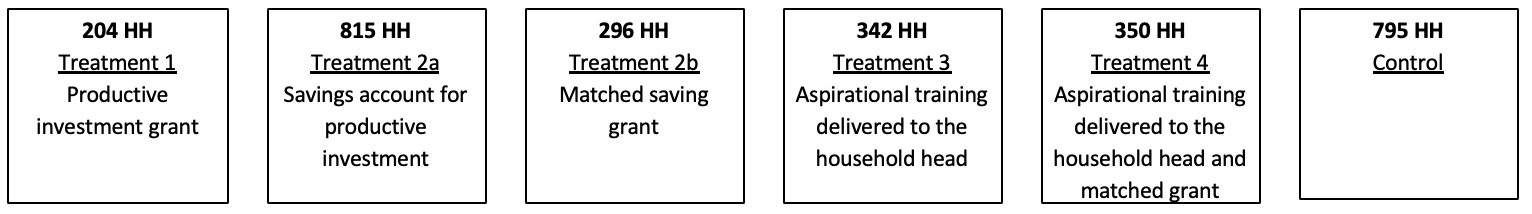
\includegraphics[width=60mm]{img/Grants4}
	\end{figure}
	
	\item<1>  Which variables should we stratify by?
			\newline - Proximity to a rehabilitated road (yes, no)
			\newline - Income (high, medium, low)
			\newline - Gender of HH head (male, female)
			\newline - Municipality (10 different municipalities)
	
	\item<1>  How many strata do we have?
	
\end{itemize}
\end{frame}


\begin{frame}{Why is this important?}

\begin{itemize}[<default overlay specification>]
	\item<1>  Transparency, transparency, transparency.
	\item<1>  There can be no doubt as to whether treatment was assigned to one household in lieu of another due to favoritism.
	\item<1>  Especially, when benefits include something like cash.
	\item<1>  This procedure is designed to be conducted in the company of government counterparts.
	\item<1> Conducting the randomization ceremony and documenting it ensure there is no doubt as to whether assignment was random.
\end{itemize}

\end{frame}


\begin{frame}{Why is this important?}

	\begin{figure}
		\centering
		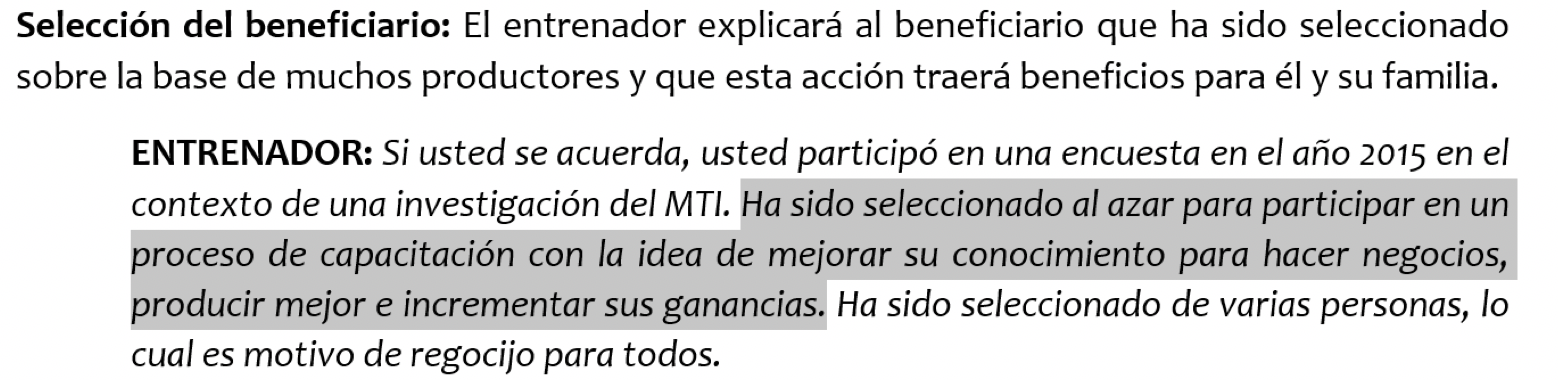
\includegraphics[width=110mm]{img/Transparency}
	\end{figure}
	
\begin{itemize}[<default overlay specification>]
	\item<1>  During visits to offer the training, we made it extremely clear that participants were chosen randomly.
\end{itemize}

\end{frame}


\begin{frame}{Randomization Procedure}
\begin{multicols}{2}	
	
	\begin{itemize}[<default overlay specification>]
		\item<1>  Assignment of 2,802 households to the 5 treatment groups and the control group.
		\item<1> Each HH has the following probabilities of being selected to receive each treatment:
			\newline - T1: Productive bonus: 200/2802 (7.1\%) (= 0)
			\newline - T2: Simple savings account: 800 / 2,802 (28.6\%) (= 1)
			\newline - T3: Account plus paired subsidy: 300 / 2,802 (10.7\%) (= 2)
			\newline - T4: Training "personal initiative": 350 / 2,802 (12.5\%) (= 3)
			\newline - T5: Account plus grant + training: 350 / 2,802 (12.5\%) (= 4)
			\newline - T6: Control: 800 / 2,802 (28.6\%) (= 5)
	   \item<1> The last two homes are assigned at random to T1-T6.
	   \item<1> Then we allocate 200/301 other homes "just in case."

	\end{itemize}
	
\end{multicols}
\end{frame}


\begin{frame}{Background}

\begin{itemize}[<default overlay specification>]
	\item<1>  Random number tables have been used for a long time. Nowadays, computational random number generators are employed.

	\item<1>  Stata’s random-number generation functions, such as uniform(), follow deterministic algorithms that are pseudorandom-number functions. 
	\item<1>  The sequences these functions produce are determined by the seed.
	\item<1>  Different seeds produce different sequences.
\end{itemize}

\end{frame}


\begin{frame}{Example: unsorted}

\begin{figure}
	\centering
	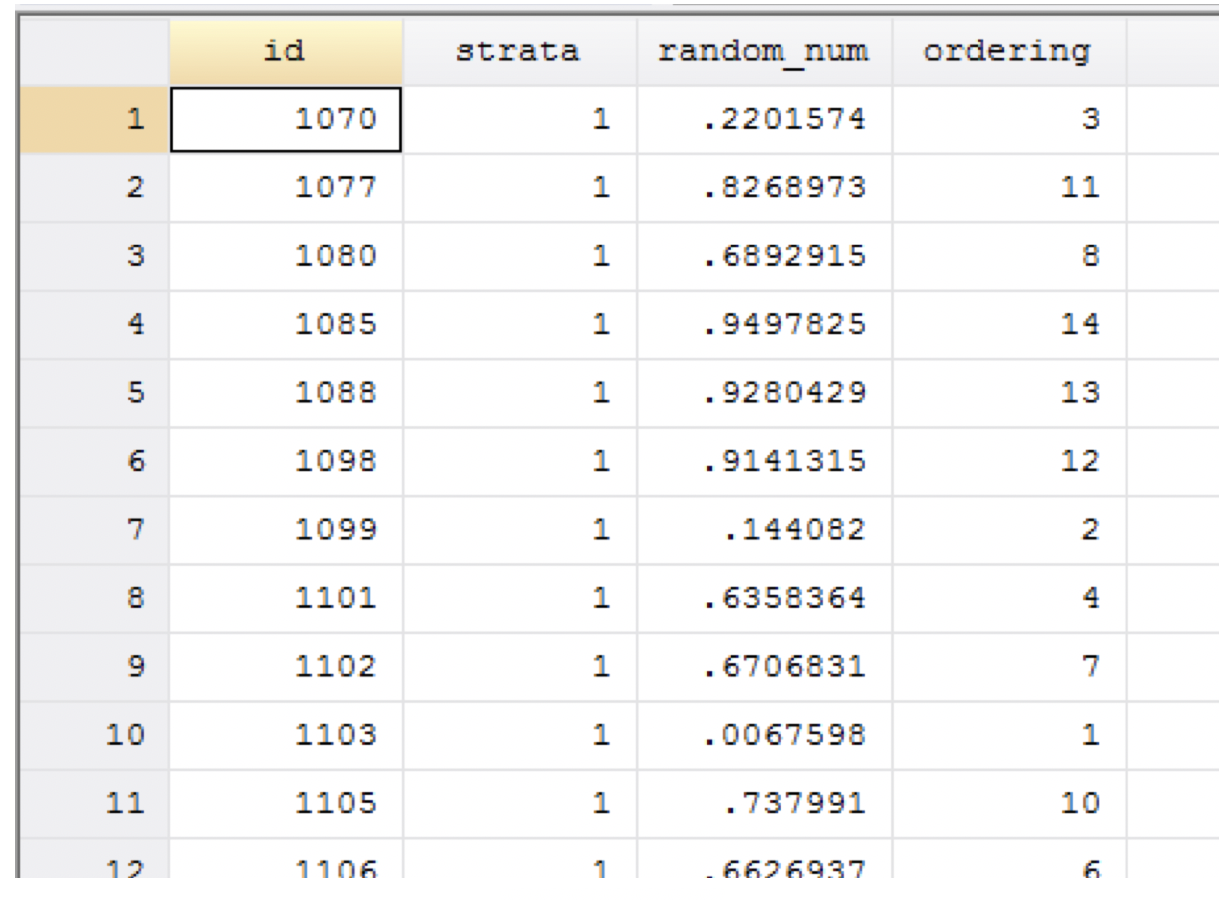
\includegraphics[width= 90mm]{img/Unsorted}
\end{figure}

\end{frame}


\begin{frame}{Example: HHs ordered according to ordering}

\begin{figure}
	\centering
	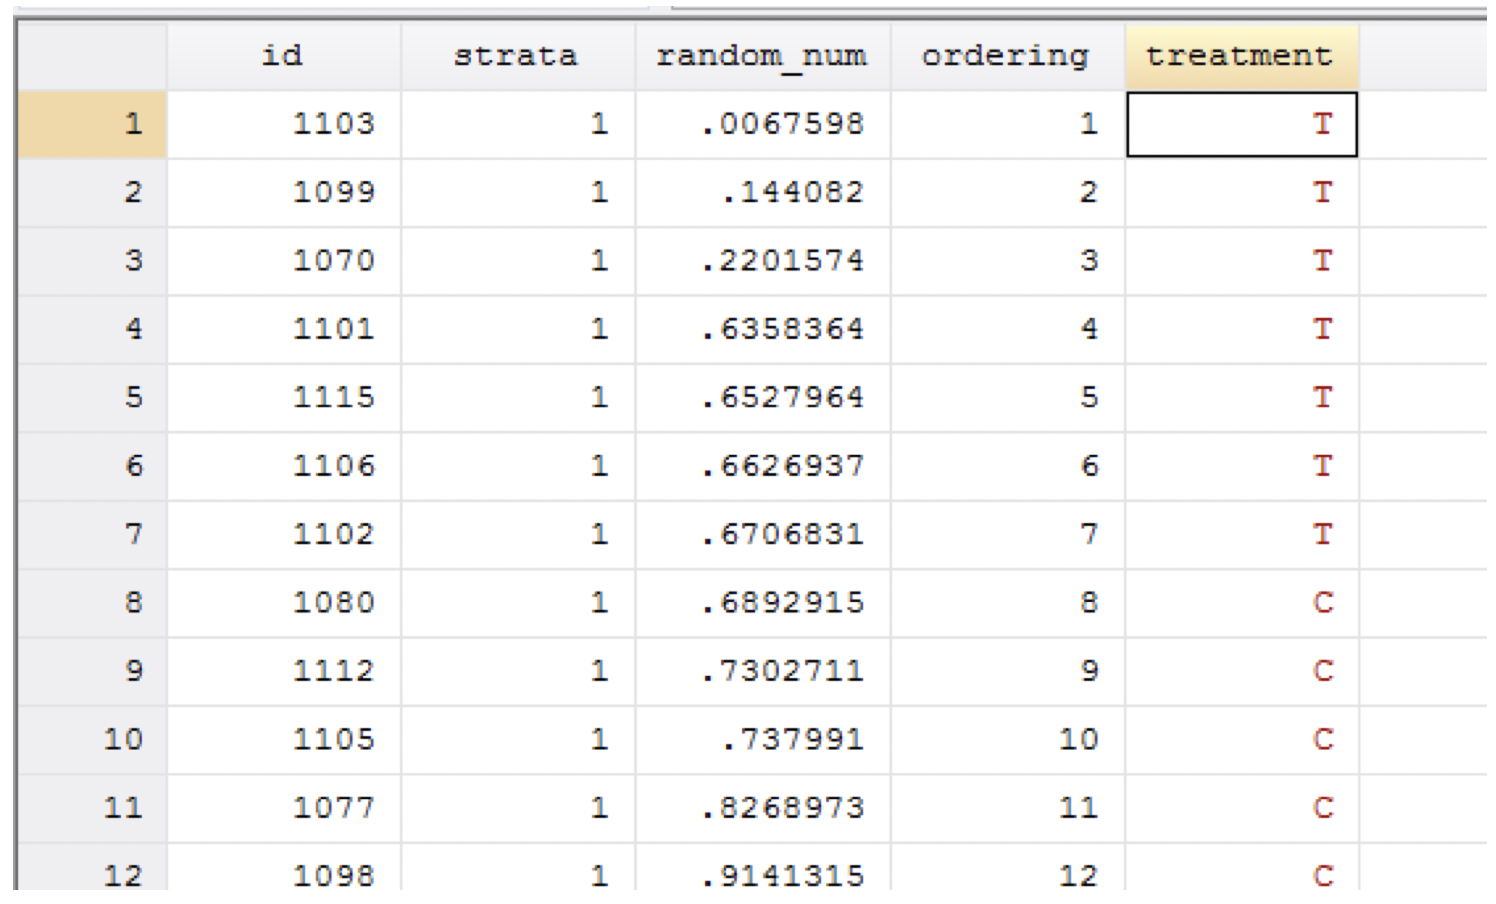
\includegraphics[width= 90mm]{img/Unsorted2}
\end{figure}

\end{frame}


\begin{frame}{Randomization in Practice}

\begin{itemize}[<default overlay specification>]
	\item<1>  We randomly draw the seed three times:
		\newline  - Actual Randomization
	\item<1>  Show that each time randomization outcome is different one from the next. 
	\item<1>  To make this easy, we will each time show results for a single household and compare afterwards.
\end{itemize}

\end{frame}

%%%%%%%%%%%%%%% Final thougts section %%%%%%%%%%%%%%%%%%%
\begin{frame}{Conclusion}

Thank you!

\vspace{20mm}
For more information or further questions please contact:
\newline Benjamin Daniels (\url{bdaniels@worldbank.org}) 

\end{frame}

%%%%%%%%%%%%%%%%%%%%%%%%%%%%%%%%%%%%%%%%%%% The End
\sectionpic{The End}{img/section_slide}






\end{document} 